\documentclass[preprint]{sigplanconf}

% The following \documentclass options may be useful:
%
% 10pt          To set in 10-point type instead of 9-point.
% 11pt          To set in 11-point type instead of 9-point.
% authoryear    To obtain author/year citation style instead of numeric.

\usepackage{amsmath}
\usepackage[T1]{fontenc}
\usepackage[utf8]{inputenc}
\usepackage[unicode=true,hidelinks]{hyperref}
\usepackage{graphicx}
\usepackage{moresize}

\usepackage{hyperref}
\usepackage{listings}
%\usepackage[scaled]{luximono}


%\usepackage{natbib}

% ----- begin macros

\lstdefinelanguage{Scala}%
{morekeywords={abstract,%
  case,catch,char,class,%
  def,else,extends,final,for,%
  if,import,implicit,%
  match,module,%
  new,null,%
  object,override,%
  package,private,protected,public,%
  for,public,return,super,%
  this,throw,trait,try,type,%
  val,var,%
  with,%
  yield,%
  lazy%
  },%
  sensitive,%
  morecomment=[l]//,%
  morecomment=[s]{/*}{*/},%
  morestring=[b]",%
  morestring=[b]',%
  showstringspaces=false%
}[keywords,comments,strings]%

\lstdefinelanguage{JavaScript}%
{morekeywords={for, var, attributes, class, classend, do, else, empty, endif, endwhile, fail, function,
functionend, if, implements, in, inherit, inout, not, of, operations, out, return,
then, types, while, use},%
  sensitive,%
  morecomment=[l]//,%
  morecomment=[s]{/*}{*/},%
  morestring=[b]",%
  morestring=[b]',%
  showstringspaces=false%
}[keywords,comments,strings]%
\lstset{language=Scala,%
  mathescape=false,%
%  columns=[c]fixed,%
  aboveskip=\smallskipamount,
  belowskip=\smallskipamount,
%  basewidth={0.5em, 0.4em},%
  basicstyle=\scriptsize,%
  captionpos=b,
  keywordstyle=\bfseries%\sffamily\bfseries,%
%  keywordstyle=\sffamily\bfseries,%
%  xleftmargin=0.5cm
}

\newcommand{\commentstyle}[1]{\slseries{#1}}
\newcommand{\keywordstyle}[1]{\bfseries{#1}}

\lstnewenvironment{slisting}{\lstset{language=Scala}}{}

\newcommand{\code}[1]{\lstinline[language=Scala,columns=fixed,basicstyle=\ttfamily\small]|#1|}

\def\changemargin#1#2{\list{}{\rightmargin#2\leftmargin#1}\item[]}
\let\endchangemargin=\endlist

%\setlength{\columnseprule}{0.25pt}

%\renewcommand{\note}[1]{$\spadesuit$ \textbf{#1} $\clubsuit$}


%\newcommand{\comment}[1]{}


\newcommand{\ie}{\emph{i.e.}}
\newcommand{\eg}{\emph{e.g.}}
\newcommand{\cf}{\emph{cf.~}}
\newcommand{\etal}{\emph{et al.~}}
\newcommand{\etc}{\emph{etc.}}
\newcommand{\aka}{\emph{a.k.a.}}


\begin{document}

\conferenceinfo{GPCE '13}{October 27--28, 2013, Indianapolis, Indiana, USA} 
\copyrightyear{2013}
\copyrightdata{[to be supplied]} 

%\titlebanner{banner above paper title}        % These are ignored unless
%\preprintfooter{short description of paper}   % 'preprint' option specified.

\title{Efficient High-Level Abstractions for Web Programming}
%\subtitle{You don’t have to trade abstraction for control}

\authorinfo{Julien Richard-Foy\and Olivier Barais\and Jean-Marc Jézéquel}
           {IRISA, Université de Rennes 1}
           {\{first\}.\{last\}@irisa.fr}

\maketitle

\begin{abstract}
%\vspace{0.2cm}


Writing large Web applications is known to be difficult. One challenge comes from the fact that the
application's logic is scattered into heterogeneous clients and servers, making it difficult to
share code between both sides or to move code from one side to the other. Another challenge is
performance: while Web applications rely on ever more code on the client-side, they may run on smart
phones with limited hardware capabilities. These two challenges raise the following problem: how to
benefit from high-level languages and libraries making code complexity easier to manage and
abstracting over the clients and servers differences without trading this engineering comfort for
performance? This article presents high-level abstractions defined as deep embedded DSLs in Scala,
that can (1) generate efficient code leveraging the target platform characteristics, (2) be shared
between clients and servers. Though code written with our DSL has a high level of abstraction our
benchmark on a real world application reports that it runs as fast as hand tuned low-level
JavaScript code.
\end{abstract}

\category{D.3.3}{Programming Languages}{Language Constructs and Features}

\terms Languages, Software Engineering

\keywords Heterogeneous code generation, Domain-specific languages, Scala, Web

\section{Introduction}

%\vspace{0.2cm}

Web applications are attractive because they require no installation or deployment steps on clients
and enable large scale collaborative experiences. However, writing large Web applications is known
to be difficult~\cite{Mikkonen08_SpaghettiJs,Preciado05_RIAMethodologyNecessity}. One challenge
comes from the fact that the business logic is scattered into heterogeneous client-side and
server-side environments~\cite{Echeverria09_RIA,Kuuskeri09_PartitioningClientServer}. This gives
less flexibility in the engineering process and requires a higher maintenance effort: there is no
way to move a piece of code targeting the server-side to target the client-side -- the code has to
be rewritten. Even worse, logic parts that run on both client-side and server-side need to be
duplicated. For instance, HTML fragments may be built from the server-side when a page is requested
by a client, but they may also be built from the client-side to perform an incremental update
subsequent to a user action. How could developers write HTML fragment definitions once and render
them on both client-side and server-side?

The more interactive the application is, the more logic needs to be duplicated between the
server-side and the client-side, and the higher is the complexity of the client-side code.
Developers can use libraries and frameworks to get high-level abstractions on client-side, making
their code easier to reason about and to maintain, but also making their code run less efficiently
due to \emph{abstraction penalty}.

Performance is a primary concern in many Web applications, because they are expected to run on a
broad range of devices, from the powerful desktop personal computer to the less powerful smart
phone~\cite{Souders08_Perf,Huang10_Perf}.

Using the same programming language on both server-side and client-side could improve the software
engineering process by enabling code reuse between both sides. Incidentally, the JavaScript language
-- which is currently the most supported action language on Web clients -- can be used on
server-side. Conversely, an increasing number of programming languages or compiler back-ends can
generate JavaScript code (\eg{} Java/GWT~\cite{Chaganti07_GWT},
SharpKit\footnote{\href{http://sharpkit.net}{http://sharpkit.net}}, Dart~\cite{Griffith11_Dart},
Kotlin\footnote{\href{http://kotlin.jetbrains.org/}{http://kotlin.jetbrains.org/}},
ClojureScript~\cite{McGranaghan11_ClojureScript},
Fay\footnote{\href{http://fay-lang.org/}{http://fay-lang.org/}},
Haxe~\cite{Cannasse08_HaXe} or Opa\footnote{\href{http://opalang.org/}{http://opalang.org/}}).

However, using the same programming language is not enough because the client and server programming
environments are not the same. For instance, DOM fragments can be defined on client-side using the
standard DOM API, but this API does not exist on server-side. How to define a common vocabulary for
such concepts? And how to make the executable code leverage the native APIs, when possible, for
performance reasons?

Generating efficient code for heterogeneous platforms is hard to achieve in an extensible way: the
translation of common abstractions like collections into their native counterpart (JavaScript arrays
on client-side and standard library's collections on server-side) may be hard-coded in the compiler,
but that approach would not scale to handle all the abstractions a complete application may use
(\eg{} HTML fragment definitions, form validation rules, or even some business data type that may be
represented differently).

On one hand, for engineering reasons, developers want to write Web applications using a single
high-level language, abstracting over the target platforms differences and reducing code complexity.
But on the other hand, for performance reasons, they want to keep control on the way their code is
compiled to each target platform. We propose to solve this dilemma by providing high-level
abstractions in compiled domain-specific embedded languages (DSELs)~\cite{Hudak96_DSEL,
Elliott2003_Compiling}. Compiled DSELs allow the definition of domain-specific languages (DSLs) as
libraries on top of a host language, and to compile them to a target platform. Their deep embedding
gives the opportunity to control the code generation scheme for a given abstraction and target
platform.

Kossakowski \etal introduced \emph{js-scala}, a compiled embedded DSL defined in Scala that
generates JavaScript code, making it possible to write the client-side code of Web applications
using JavaScript~\cite{Kossakowski12_JsDESL}. However, Kossakowski \etal did not address the
engineering dilemma described above. This paper enriches js-scala with the following
contributions\footnote{The code is available at
\href{http://github.com/js-scala}{http://github.com/js-scala}}:

\begin{itemize}
 \item we define high-level abstractions, typically used in Web programming, that generate low-level
code leveraging native Web browser APIs;
 \item in the case of abstractions shared between servers and clients, we specialize the code
generation in order to leverage the target platform native environments.
\end{itemize}

We validate our approach with a case study implemented with various candidate technologies and
discuss the relative pro and cons of them. Though the code written in our DSL is high-level and can
be shared between clients and servers, it has the same runtime performances on client-side as
hand-tuned low-level JavaScript code.

The remainder of this paper is organized as follows. The next section overviews the
existing approaches defining high-level languages for Web programming. Section \ref{sec:lms}
presents the framework we used to define our DSLs. Section \ref{sec:contribution} presents our
contribution. Section \ref{sec:validation} compares our solution to common approaches. Section
\ref{sec:conclusion} discusses our results and concludes.

\section{Related Work}
\label{sec:related-work}


%\vspace{0.1cm}

We classified existing approaches providing high-level abstractions for Web programming in four
categories, as shown in figure \ref{fig:langs}.

\begin{figure}[htb]
\begin{center}
\includegraphics[width=7.5cm]{langs.pdf}
\end{center}
\caption{Language engineering processes}
\vspace{-0.5cm}
\label{fig:langs}
\end{figure}

\paragraph{Fat Languages}

%\vspace{0.1cm}

The first approach for defining a cross-platform language consists in hard-coding, in the compiler,
the code generation scheme of each language feature to each target platform. Figure \ref{fig:langs}
(a) depicts this process. In order to support a feature related to a specific domain, the whole
compiler pipeline (parser, code generator, \etc) may have to be adapted. This approach gives
\emph{fat} languages because a lot of concepts are defined at the language level: general
programming concepts such as naming, functions, classes, as well as more domain-specific concepts
such as HTML fragment definition. Thus, implementing a fat language may require a high effort.
Examples of such languages for Web programming are Links~\cite{Cooper07_Links}, Opa and
Dart~\cite{Griffith11_Dart}.

\paragraph{Domain-Specific Languages}

%\vspace{0.1cm}

Another approach consists in defining several independent domain-specific
languages~\cite{Van00_DSL}, each one focusing on concerns specific to a given problem domain, and
then to combine all the source artifacts written with these language into one executable program, as
shown in figure~\ref{fig:langs} (b). Defining such languages requires a minimal effort compared to
the previous approach because each language has a limited set of features. On the other hand, it is
difficult to have interoperability between DSLs. \cite{Groenewegen08_WebDSL} gave an example of such
a domain-specific language for defining Web applications.

\paragraph{Thin Languages}

%\vspace{0.1cm}

Alternatively, one can define concepts relative to a specific domain as a library on top of a thin
general purpose language (it is also referred to as a domain-specific \emph{embedded}
language~\cite{Hudak96_DSEL}). Figure \ref{fig:langs} (c) depicts this approach. Defining such a
library requires minimal effort (though the syntax of the DSL is limited by the syntax flexibility
of the host language) and several DSLs can interoperate freely within the host language. However,
this approach gives no opportunity to efficiently translate a concept according to the target
platform characteristics because the compiler has no domain-specific knowledge (though some
compilers hard-code the translation of some common abstractions such as arrays to leverage the
target platform characteristics). Examples of languages following this approach are Java/GWT,
Kotlin, HaXe and SharpKit.

\paragraph{Deeply Embedded Languages}

%\vspace{0.1cm}
The last approach, shown in figure \ref{fig:langs} (d), can be seen as a middle-ground between the
two previous approaches: DSLs are embedded in a host language but use a code generation process.
This approach shares the same benefits and limitations as embedded DSLs for defining language units.
However, the code generation process is specific to each DSL and gives the opportunity to perform
domain-specific optimizations. In other words deeply embedded DSLs bring domain-specific knowledge
to the compiler. Js-scala~\cite{Kossakowski12_JsDESL} is an example of deeply embedded DSL in Scala
for Web programming. It makes it possible to produce JavaScript programs from Scala code that uses
basic language concepts like arrays and control structures (\code{if} and \code{while}) as well as
mechanisms specific to the Scala compiler, like delimited continuations to handle asynchronous
computations. Though the initial authors of js-scala showed how to use the native browser APIs in an
untyped fashion, they did not show how to build high-level abstractions for Web programming
generating efficient code leveraging the browser APIs and did not show how to share such
abstractions between server and client sides (they achieved code sharing, yet on the server-side
their DSL was not compiled but interpreted). Our paper addresses these limitations.

\section{Lightweight Modular Staging}
\label{sec:lms}

This section gives background material on the framework used to define js-scala.

Lightweight Modular Staging~\cite{Rompf12_LMSThesis, Rompf12_LMS} (LMS) is a framework for defining
deeply embedded DSLs in Scala. It has been used to define high-performance DSLs for parallel
computing~\cite{Brown11_Parallel} and to define JavaScript as an embedded DSL in
Scala~\cite{Kossakowski12_JsDESL}.

LMS is based on staging~\cite{Jorring1986_Staging}: a program using LMS is a regular Scala program
that evaluates to an intermediate representation (IR) of a final program. This IR is a graph of
expressions that can be traversed by code generators to produce the final program code. Expressions
evaluated in the initial program and those evaluated in the final program (namely, staged
expressions) are distinguished by their type: a \code{Rep[Int]} value in the initial program is a
staged expression that generates code evaluating to an \code{Int} value in the final program. An
\code{Int} computation in the initial program is evaluated during the initial program evaluation and
becomes a constant in the final program.

Defining a DSL with LMS consists in the following steps:

\begin{itemize}
 \item writing a Scala module providing the DSL vocabulary as an abstract API,
 \item implementing the API in terms of IR nodes,
 \item defining a code generator visiting IR nodes and generating the corresponding code.
\end{itemize}

\section{Efficient High-Level Abstractions for Web Programming}
\label{sec:contribution}

This section presents some tasks typically performed in Web applications, either on client-side or
server-side or on both, generalizes them in terms of high-level abstractions, and shows how they are
implemented in js-scala to generate efficient code.

\subsection{Selectors API}
\label{sec:selectors}

In a Web application, the user interface is defined by a HTML document that can be updated by the
JavaScript code. A typical operation consists in searching some “interesting” element in the
document, in order to extract its content, replace it or listen to user events triggered on it (such
as mouse clicks). The standard API provides several functions to search elements in a HTML document
according to their name or attribute values. Figure~\ref{selectors-api} summarizes the available
functions and their differences.

\begin{figure}[htb]
\begin{center}
\begin{tabular}{| l | p{3cm} |}
\hline
Function & Description \\
\hline
\code{querySelector(s)} & First element matching the CSS selector \code{s} \\
\hline
\code{getElementById(i)} & Element which attribute \code{id} equals to \code{i} \\
\hline
\code{querySelectorAll(s)} & All elements matching the CSS selector \code{s} \\
\hline
\code{getElementsByTagName(n)} & All elements of type \code{n} \\
\hline
\code{getElementsByClassName(c)} & All elements which \code{class} attribute contains \code{c} \\
\hline
\end{tabular}
\end{center}
\caption{Standard selectors API. The \code{querySelector} and \code{querySelectorAll} are the most
general functions while the others handle special cases.}
\label{selectors-api}
\end{figure}

\begin{figure}[htb]
\begin{lstlisting}[language=JavaScript,label=vanilla-selectors,caption=Searching elements using the
native selectors API]
function getWords() {
  var form = document.getElementById('add-user');
  var sections =
    form.getElementsByTagName('fieldset');
  var results = [];
  for (var i = 0 ; i < sections.length ; i++) {
    var words = sections[i]
      .getElementsByClassName('word');
    results[i] = words;
  }
  return results
}
\end{lstlisting}
\end{figure}

Listing \ref{vanilla-selectors} gives an example of use of various functions from the native
selectors API to retrieve a list of input fields within a form. The existence of several
specialized functions in the API makes it possible to write efficient code, but forces users to
think at a low abstraction level.

\begin{figure}[htb]
\begin{lstlisting}[language=JavaScript,label=jquery-selectors,caption=Searching elements in jQuery]
function getWords() {
  var form = $('#add-user');
  var sections = $('fieldset', form);
  return sections.map(function () {
    return $('.word', this)
  })
}
\end{lstlisting}
\end{figure}

A high-level abstraction for searching elements in a document could be just one function
finding all elements matching a given CSS selector. In fact, most JavaScript
developers\footnote{According to
\href{http://trends.builtwith.com/javascript}{http://trends.builtwith.com/javascript}, jQuery is
used by more than 40\% of the top million sites.} use the jQuery library~\cite{Bibeault08_jQuery}
that actually provides only one function to search for elements. Listing \ref{jquery-selectors}
shows an equivalent JavaScript program as listing \ref{vanilla-selectors}, but using jQuery. The
code is both shorter and simpler, thanks to its higher-level of abstraction. jQuery provides an API
that is simpler to master because it has less functions, but this benefit comes at the price of a
decrease in runtime performances.

Instead, we propose a solution that has a high-level API but generates JavaScript code using the
specialized native API, when possible, in order to get both engineering comfort and performances.
We achieve this by analyzing, during the first evaluation step, the selector that is
passed as parameter and, when appropriate, by producing JavaScript code using the specialized API,
and otherwise producing code using \code{querySelector} and \code{querySelectorAll}.

\begin{figure}[htb]
\begin{lstlisting}[label=selector-impl,caption=Selectors optimization]
def find(selector: Rep[String]) =
  getConstIdCss(selector) match {
    case Some(id) if receiver == document =>
      DocumentGetElementById(Const(id))
    case _ =>
      SelectorFind(receiver, selector)
  }
\end{lstlisting}
\end{figure}

Our API has two functions: \code{find} to find the first element matching a selector and
\code{findAll} to find all the matching elements. Listing \ref{selector-impl} gives the
implementation of the \code{find} function. It is a Scala function that returns an IR node
representing the JavaScript computation that will search the element in the final program. The
\code{getConstIdCss} function analyzes the selector: if it is a constant \code{String} value
containing a CSS ID selector, it returns the value of the identifier. So, if the \code{find}
function is applied to the \code{document} and to an ID selector, it returns a
\code{DocumentGetElementById} IR node (that is translated to a \code{document.getElementById} call
by the code generator), otherwise it returns a \code{SelectorFind} IR node (that is translated to a
\code{querySelector} call).

The same applies to the implementation of \code{findAll}: the selector passed as parameter is
analyzed and the function returns a \code{SelectorGetElementsByClassName} in case of a CSS class
name selector, a \code{SelectorGetElementsByTagName} in case of a CSS tag name selector, and a
\code{SelectorFindAll} otherwise.

\begin{figure}[htb]
\begin{lstlisting}[label=js-scala-selectors,caption=Searching elements in js-scala]
def getWords() = {
  val form = document.find("#add-user")
  val sections = form.findAll("fieldset")
  sections map (_.findAll(".word"))
}
\end{lstlisting}
\end{figure}

\begin{figure}[htb]
\begin{center}
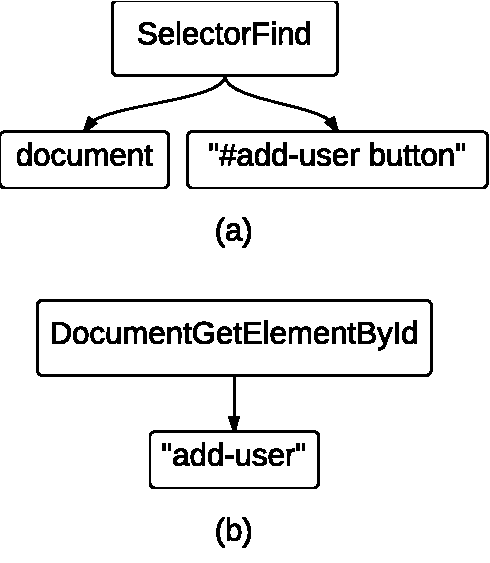
\includegraphics[width=5cm]{ir.pdf}
\end{center}
\caption{Intermediate representations returned by the evaluation of (a)
\code{document.find("\#add-user button")} and (b) \code{document.find("\#add-user")}}
\label{fig:ir}
\end{figure}

\vspace{1 cm}

Figure \ref{fig:ir} shows the IRs returned by the evaluation of \small{
$document\\.find("\#add-user button")$} \normalsize{and}  \small{$ document.find("\#add-user")$}.

\normalsize{}

\sloppy
In the former case, the selector is parsed and does not match an ID selector (it is a composite
selector matching button elements within the element having the \code{add-user} id), so a
\code{SelectorFind} node is returned, then translated into a call to the general
\code{querySelector} function. In the latter case, the selector matches an ID selector so a
\code{DocumentGetElementById} node is returned, then translated into a call to the specialized
\code{getElementById} function.

Finally, listing~\ref{js-scala-selectors} shows how to implement listing~\ref{jquery-selectors} in
Scala using js-scala. The code has the same abstraction level as with jQuery, however it
generates a JavaScript program identical to listing~\ref{vanilla-selectors}: the high-level
abstractions (the \code{find} and \code{findAll} functions) exist only in the initial program, not
in the final JavaScript program.

\subsection{Monads Sequencing}
\label{sec:option}

This section presents an abstraction to handle \code{null} references and shows how this
abstraction can be shared between client and server code.

\code{null} references are a known source of problems in programming
languages~\cite{Hoare09_Null,Nanda09_Null}. For example, consider listing \ref{null-unsafe} finding
a particular widget in the page and then a particular button within the widget. The native
\code{querySelector} method returns \code{null} if no node matched the given selector in the
document. If we run this code in a page where the widget is not present, it will throw an error
and stop further JavaScript execution. Defensive code can be written to handle \code{null}
references, but leads to very cumbersome code, as shown in listing \ref{null-defensive}.

\begin{figure}[htb]
\begin{lstlisting}[language=JavaScript,label=null-unsafe,caption=Unsafe code]
var loginWidget =
  document.querySelector("div.login");
var loginButton =
  loginWidget.querySelector("button.submit");
loginButton.addEventListener("click", handler);
\end{lstlisting}
\end{figure}


\begin{figure}[htb]
\begin{lstlisting}[language=JavaScript,label=null-defensive,caption=Defensive programming to handle
null references]
var loginWidget =
  document.querySelector("div.login");
if (loginWidget !== null) {
  var loginButton =
    loginWidget.querySelector("button.submit");
  if (loginButton !== null) {
    loginButton.
      addEventListener("click", handler);
  }
}
\end{lstlisting}
\end{figure}

Some programming languages encode optional values with a monad (\eg{} \code{Maybe} in Haskell and
\code{Option} in Scala). In that case, sequencing over the monad encodes optional value
dereferencing. If the language supports a convenient syntax for monad sequencing, it brings a
convenient syntax for optional value dereferencing, alleviating developers from the burden of
defensive programming.

In our DSL, we encode an optional value of type \code{Rep[A]} using a \code{Rep[Option[A]]} value,
which can either be a \code{Rep[Some[A]]} (if there is a value) or a \code{Rep[None.type]} (if
there is no value). An optional value can be dereferenced using the \code{for} notation, as shown
in listing \ref{null-js-scala}, that implements in js-scala a program equivalent to listing
\ref{null-defensive}. The \code{find} function returns a \code{Rep[Option[Element]]}. The \code{for}
expression contains a sequence of statements that are executed in order, as long as the previous
statement returned a \code{Rep[Some[Element]]} value.

\begin{figure}[htb]
\begin{lstlisting}[label=null-js-scala,caption=Handling null references in js-scala]
for {
  loginWidget <- document.find("div.login")
  loginButton <- loginWidget.find("submit.button")
} loginButton.on(Click)(handler)
\end{lstlisting}
\end{figure}

Such a monadic API brings both safety and expressiveness to developers manipulating optional values
but usually involves the creation of an extra container object holding the optional value. In our
case, the monadic API is used in the initial program but generates code that does not wrap values in
container objects but instead checks if they are \code{null} or not when dereferenced. So the extra
container object exists only in the initial program and is removed during code generation: listing
\ref{null-js-scala} produces a code equivalent to listing~\ref{null-defensive}.

\begin{figure}[htb]
\begin{lstlisting}[caption=JavaScript code generator for null references handling
DSL,label=option-codegen,captionpos=b]
override def emitNode(sym: Sym[Any], rhs: Def[Any]) =
  rhs match {
    case OptionIsEmpty(o) =>
      emitValDef(sym, q" $o === null")
    case OptionForeach(o, b) =>
      stream.println(q"if ($o !== null) {")
      emitBlock(b)
      stream.println("}")
    case _ =>
      super.emitNode(sym, rhs)
  }
\end{lstlisting}
\end{figure}

Listing \ref{option-codegen} shows the JavaScript code generator for methods \code{isEmpty} (that
checks if the optional value contains a value) and \code{foreach} (that is called when the
\code{for} notation is used, as in listing \ref{null-js-scala}). The \code{emitNode} method handles
\code{OptionIsEmpty} and \code{OptionForeach} nodes returned by the implementations of
\code{isEmpty} and \code{foreach}, respectively. In the case of the \code{OptionIsEmpty} node, it
simply generates an expression testing if the value is \code{null}. In the case of the
\code{OptionForeach} node, it wraps the code block dereferencing the value within a \code{if}
checking that the value is not \code{null}.

The IR nodes are not tied to the JavaScript code generator, so we are able to make this abstraction
available on server-side by writing a code generator similar to the JavaScript code generator, but
targeting Scala. So the same abstraction is efficiently translated on both server and client sides.

\subsection{DOM Fragments Definition}
\label{sec:forest}

This section shows how we define an abstraction shared between clients and servers, as in the
previous section, but that has different native counterparts on client and server sides. The
challenge is to define an API providing a common vocabulary that generates code using the target
platform native APIs.

\begin{figure}[htb]
\begin{lstlisting}[language=JavaScript,caption=JavaScript DOM API,label=dom-api]
var articleUi = function (article) {
  var div = document.createElement('div');
  div.setAttribute('class', 'article');
  var span = document.createElement('span');
  var name =
    document.createTextNode(article.name + ': ');
  span.appendChild(name);
  div.appendChild(span);
  var strong = document.createElement('strong');
  var price = document.createTextNode(article.price);
  strong.appendChild(price);
  div.appendChild(strong);
  return div
};
\end{lstlisting}
\end{figure}

\begin{figure}[htb]
\begin{lstlisting}[caption=Scala XML API,label=scala-xml-api]
def articleUi(article: Article) =
  <div class="article">
    <span>{ article.name + ": " }</span>
    <strong>{ article.price }</strong>
  </div>
\end{lstlisting}
\end{figure}

A common task in Web applications consists in computing HTML fragments representing a part of the
page content. This task can be performed either from the server-side (to initially respond to a
request) or from the client-side (to update the current page). As an example, listing \ref{dom-api}
defines a JavaScript function \code{articleUi} that builds a DOM tree containing an article
description, and listing \ref{scala-xml-api} shows how one could implement a similar function on
server-side using the standard Scala XML library. The reader may notice that the client-side
and server-side APIs are very different and that the client-side API is very low-level and
inconvenient to use.

Our first step consists in capturing, in a high-level API, the concepts common to the JavaScript and
Scala APIs. Though they are different, both APIs define HTML elements with attributes and content.
We propose to have a function \code{el} to define an HTML element, eventually containing attributes
and children elements. Any children of an element that is not an element itself is converted into a
text node. Listing \ref{forest} shows how to implement our example with our DSL. The children
elements of an element can also be obtained dynamically from a collection, as shown in listing
\ref{forest-loops}.

\begin{figure}[htb]
\begin{lstlisting}[label=forest,caption=DOM definition DSL]
def articleUi(article: Rep[Article]) =
    el('div, 'class -> 'article)(
        el('span)(article.name + ": "),
        el('strong)(article.price)
    )
\end{lstlisting}
\end{figure}

\begin{figure}[htb]
\begin{lstlisting}[label=forest-loops,caption=Using loops]
def articlesUi(articles: Rep[Seq[Article]]) =
    el('ul)(
        for (article <- articles)
        yield el('li)(articleUi(article))
    )
\end{lstlisting}
\end{figure}

The \code{el} function returns an \code{Element} IR node that is a tree composed of other
\code{Element} and \code{Text} nodes. The JavaScript and Scala code generators traverse this tree
and produce code building an equivalent DOM tree and XML fragment, respectively. When the children
of an element are constant values (as in listing \ref{forest}) rather than dynamically computed (as
in listing \ref{forest-loops}), the code generators unroll the loop that adds children to their
parent, for better performance. As a result, listing \ref{forest} generates a code equivalent to
listing \ref{dom-api} on client-side and equivalent to listing \ref{scala-xml-api} on server-side.

\begin{figure*}
\begin{lstlisting}[language=JavaScript,label=js-gen-forest,caption=JavaScript code generator for the
DOM fragment definition DSL]
case Tag(name, children, attrs) =>
  emitValDef(sym, q"document.createElement('$name')")
  for ((n, v) <- attrs) {
    stream.println(q"$sym.setAttribute('$n', $v);")
  }
  children match {
    case Left(children) =>
      for (child <- children) {
        stream.println(q"$sym.appendChild($child);")
      }
    case Right(children) =>
      val x = fresh[Int]
      stream.println(q"for (var $x = 0; $x < $children.length; $x++) {")
      stream.println(q"$sym.appendChild($children[$x]);")
      stream.println("}")
  }
case Text(content) =>
  emitValDef(sym, q"document.createTextNode($content)")
\end{lstlisting}
\end{figure*}

\begin{figure*}
\begin{lstlisting}[label=scala-gen-forest,caption=Scala code generator for the DOM fragment
definition DSL]
case Tag(name, children, attrs) =>
  val attrsFormatted =
    (for ((name, value) <- attrs)
     yield q" $name={ $value }").mkString
  children match {
    case Left(children) =>
      if (children.isEmpty) {
        emitValDef(sym, q"<$name$attrsFormatted />")
      } else {
        emitValDef(sym,
          q"<name$attrsFormatted>{ ${children.map(quote)} }</$name>"
        )
      }
    case Right(children) =>
      emitValDef(sym, q"<$name$attrsFormatted>{ $children }</$name>")
  }
case Text(content) =>
  emitValDef(sym, q"{xml.Text(content)}")
\end{lstlisting}
\end{figure*}

Listings \ref{js-gen-forest} and \ref{scala-gen-forest} show the relevant parts of the code
generators for this DSL. They basically follow the same pattern: they visit \code{Tag} and
\code{Text} IR nodes and produce the corresponding elements in the target language.


\section{Evaluation}
\label{sec:validation}

Our goal is to evaluate the level of abstraction provided by our solution and its performances, by
comparing it with common approaches. We take the number of lines of code as an inverse approximation
of the level of abstraction. We also evaluate the ability to share code between client and server
sides.

We realized two micro-benchmarks involving programs using the selectors DSL and the
optional value DSL, and we benchmarked a real world program. In each case we have written several
implementations of the program, using plain JavaScript, Java/GWT, HaXe and js-scala (in each case we
tried to write the application in an idiomatic way). The performance benchmarks measured the
execution time of the generated JavaScript code. The tests were executed on a DELL Latitude E6430
laptop with 8 GB of RAM, on the Google Chrome v27 Web browser.

\subsection{Micro-Benchmarks}

The micro-benchmarks measure the performance of our implementation of the selectors and optional
value abstractions.

\subsubsection{Selectors}

We could not implement this abstraction in GWT or HaXe as efficiently as we did in js-scala because
it relies on the staging mechanism: the best we could do in GWT or Haxe is to expose the native
high-level API (\code{querySelector} and \code{querySelectorAll}). So we directly compared the
execution time of the JavaScript code generated by listing \ref{js-scala-selectors} with a
JavaScript program equivalent to listing \ref{vanilla-selectors} but using the high-level native
API (\code{querySelector} and \code{querySelectorAll}) instead. The code was executed in a Web page
containing a few elements: 4 \code{fieldset} elements, each containing 0 to 2 elements with class
\code{word}.

\begin{figure}
\centering
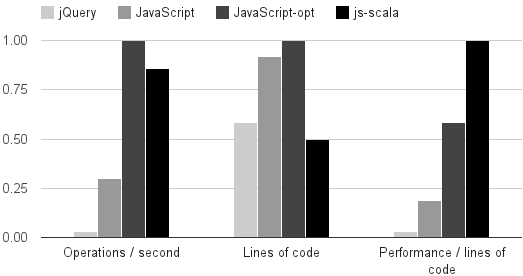
\includegraphics[width=8cm]{selectors-benchmark.png}
\caption{Micro-benchmark on the selectors abstraction}
\label{fig:selectors-benchmark}
\end{figure}

Figure \ref{fig:selectors-benchmark} shows the benchmark results. The JavaScript-opt version is
listing \ref{vanilla-selectors}, which uses low-level native APIs, the JavaScript version is the
equivalent listing using the high-level native API, and the jQuery version is listing
\ref{jquery-selectors}. The js-scala version is slightly slower than the JavaScript-opt (by 14\%),
but is 2.88 times faster than the JavaScript version, and 28.6 times faster than the jQuery
version. Finally, the js-scala version has a performance to lines of code ratio more than 1.72
times higher than others.

\subsubsection{Optional Value}

We reimplemented the optional value abstraction in plain JavaScript, Java and HaXe and wrote a small
program manipulating optional values.

\begin{figure}
\centering
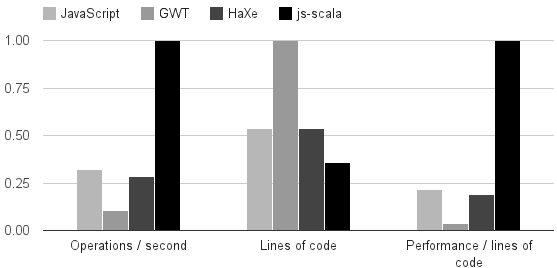
\includegraphics[width=8cm]{microbenchmark.png}
\caption{Micro-benchmark on the optional values abstraction}
\label{micro-benchmark}
\end{figure}

Figure \ref{micro-benchmark} shows the benchmark results. The js-scala version of the program runs
between 3 to 10 times faster than other approaches. This version also takes less lines of code than
others (this result is almost due to the special \code{for} notation, that has no equivalent in
other benchmarked languages). Finally, the js-scala program has a performance to lines of code ratio
more than 4 times higher than others.

\subsection{Real World Application}

Chooze~\footnote{Source code is available at
\href{http://github.com/julienrf/chooze}{http://github.com/julienrf/chooze}} is an existing
complete application for making polls. It allows users to create a poll, define the choice
alternatives, share the poll, vote and look at the results. It contains JavaScript code to handle
the dynamic behavior of the application: double-posting prevention, dynamic form update and rich
interaction with the document.

The application was initially written using jQuery. We rewrote it in vanilla JavaScript (low-level
hand-tuned code without third-party library), js-scala, GWT and HaXe.

\subsubsection{Performance}

The benchmark code simulates user actions on a Web page (2000 clicks on buttons, triggering a
dynamic update of the page and involving the use of the optional value monad, the selectors API and
the HTML fragment definition API). Figure \ref{benchmark} shows the benchmark results.

\begin{figure}
\centering
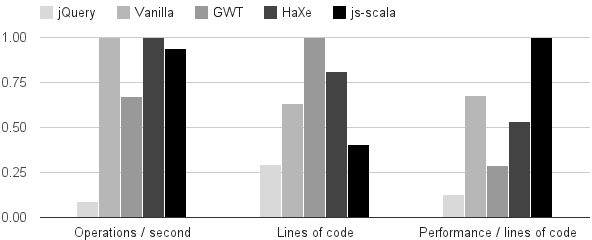
\includegraphics[width=8cm]{chooze.png}
\caption{Benchmarks on a real application}
\label{benchmark}
\end{figure}

The runtime performances of the vanilla JavaScript, HaXe and js-scala versions are similar (though
the js-scala version is slightly slower by 6\%). It is worth noting that the vanilla JavaScript and
the HaXe versions use low-level code compared to js-scala, as shown in the middle of the figure
(lines of code): the js-scala version needs only 74 lines of code while the vanilla JavaScript
version needs 116 lines of code (57\% bigger) and the HaXe version needs 148 lines of code (100\%
bigger). The jQuery JavaScript version, which code is high-level (54 lines of code, 27\% less
than js-scala) runs 10 times slower than the js-scala version.

The last part of the figure compares the runtime performance to lines of code ratio. Js-scala shows
the best score, being 1.48 times better than the vanilla JavaScript version, 1.88 times better than
the HaXe version, 3.45 times better than the GWT version and 7.82 times better than the jQuery
JavaScript version.

\subsubsection{Code Reuse}

We were able to share some DOM fragment definitions between server-side and client-side only in
the js-scala version. In the GWT version we don’t have choice: dynamic DOM fragments are always
built only on client-side (a practice that makes it more difficult to make the pages content
crawlable by search engines and may increase the initial display time). In the other versions the
code for building the DOM fragment is duplicated between client and server sides, representing 20
lines of JavaScript code (17\% of the total) and 15 lines of HTML (5\% of the total) in the
JavaScript version, and 19 lines of HaXe code (13\% of the total) and 15 lines of HTML (5\%
of the total) in the HaXe version. In the js-scala version the DOM fragment definitions shared
between clients and servers represent 22 lines of Scala code (30\% of the total) and save 15 lines
of HTML (5\% of the total).

\subsubsection{Threats to Validaty}

Our goal was to put the runtime performances in perspective with the level of abstraction. We are
aware that the indicator we chose as an inverse approximation of the abstraction level, the number
of lines of code, is not scientifically established and may be subject to discussion. However, we
think it is a reasonable approximation in our case because all the candidate languages we use have
a similar syntax, inherited from the imperative programming language.

Another weakness of our validation may come from the fact that our application does not make a
heavy use of client-side code and thus may not be representative of the way large Web applications
are written. However, we think that a richer application would have more parts of code susceptible
to be shared between client and server sides, thus giving even better results on the code reuse
statistics.



Finally, the GWT version may not have been written in an as idiomatic as possible way.

\section{Discussion}
\label{sec:conclusion}

We implemented our solution as compiled embedded DSLs in Scala. Generating code from our DSLs is a
two steps process: an initial Scala program first evaluates to an intermediate representation of
the final program that is traversed by code generators to produce the final JavaScript code.
Domain-specific optimizations can happen during the IR construction (as shown in section
\ref{sec:selectors}) or during the code generation (as shown in section \ref{sec:option}).

An important consequence of the implementation as compiled embedded DSLs is that defining a DSL
that can be shared between server and client sides requires a low effort: compiled embedded DSLs are
simply defined as libraries but let developers specialize the generated code according to each
target platform (as shown in section \ref{sec:forest}).

In other words, the compiled embedded DSL approach gives us a way to exploit the Scala host language
to define high-level language units that integrate seamlessly together and bring domain-specific
knowledge to the code generation scheme to produce efficient code for client and server sides.

These characteristics allowed us to capture some Web programming patterns as high-level
abstractions, making the code of our application simpler to reason about and making some parts of
the code reusable between client and server sides, while keeping execution performances on
client-side as high as if we used hand-tuned low-level JavaScript code.

%\appendix
%\section{Appendix Title}
%
%This is the text of the appendix, if you need one.
%
%\acks
%
%This work was funded by Zenexity.

\bibliographystyle{abbrvnat}
\bibliography{biblio}
%\begin{thebibliography}{}
%\softraggedright
%
%\bibitem[Smith et~al.(2009)Smith, Jones]{smith02}
%P. Q. Smith, and X. Y. Jones. ...reference text...
%
%\end{thebibliography}
%
\end{document}
